\documentclass[aspectratio=169,11pt]{beamer}
\usepackage{graphicx,booktabs,xcolor,amsmath,tikz}
\usetikzlibrary{arrows.meta,positioning}
\usetheme{default}
\setbeamertemplate{navigation symbols}{}
\setbeamertemplate{footline}[frame number]
\definecolor{ink}{HTML}{1A202C}
\definecolor{acc}{HTML}{2B6CB0}
\definecolor{warn}{HTML}{C53030}
\definecolor{good}{HTML}{2F855A}
\definecolor{mut}{HTML}{718096}
\setbeamercolor{structure}{fg=acc}
\setbeamercolor{normal text}{fg=ink}
\setbeamerfont{frametitle}{size=\large,series=\bfseries}
\setbeamertemplate{frametitle}{\vspace{6pt}\insertframetitle\par
  \vspace{-4pt}{\color{acc}\rule{\textwidth}{1pt}}}
\setbeamertemplate{itemize item}{\color{acc}\textbullet}
\setbeamertemplate{itemize subitem}{\color{mut}--}
\graphicspath{{../../results/figures/}}
\newcommand{\Hi}[1]{{\color{acc}\textbf{#1}}}
\newcommand{\Bad}[1]{{\color{warn}\textbf{#1}}}
\newcommand{\Good}[1]{{\color{good}\textbf{#1}}}

\title{\textbf{Measuring Multilingual Representation Quality}}
\subtitle{What a controlled study showed, and the metric that came out
of it}
\author{Waiz Khan}
\institute{\small Johns Hopkins University \quad wkhan12@jh.edu}
\date{\small August 2026}

\begin{document}

{\setbeamertemplate{footline}{}
\begin{frame}\titlepage\end{frame}}

% ---------------------------------------------------------------- 1
\begin{frame}{The question Aim 1 asks}
\large
\begin{itemize}\setlength\itemsep{10pt}
\item How strongly does a model's internal representation encode
\emph{which language} a sentence is in, rather than \emph{what it
means}?
\item Is the mapping between one language's space and another's just
linear, or more complex?
\item Can we build an intrinsic measure, computed from representations
alone, that predicts how a model actually performs?
\end{itemize}
\vspace{10pt}
{\color{mut}The third question is the hard one. An intrinsic measure is
only worth having if it is right when it matters.}
\end{frame}

% ---------------------------------------------------------------- 2
\begin{frame}{The measure we started with: LFS}
A model is given the \emph{same} 300 sentences in 41 languages. Each
sentence becomes a vector. Two things drive where those vectors sit:
\vspace{6pt}
\begin{itemize}
\item \Hi{Meaning}: which of the 300 sentences it is
\item \Hi{Language}: which of the 41 languages it is written in
\end{itemize}
\vspace{8pt}
A variance decomposition separates the two, giving
\[
\text{LFS} \;=\; \frac{\sigma^2_{\text{language}}}
{\sigma^2_{\text{language}} + \sigma^2_{\text{meaning}}}
\]
\vspace{-4pt}
\begin{itemize}
\item Low LFS means the space is organised by meaning, and language
identity has been largely factored out. That was taken to be good.
\end{itemize}
\end{frame}

% ---------------------------------------------------------------- 3
\begin{frame}{You cannot validate a metric on pretrained models alone}
\large
No pretrained model comes with a label saying how much meaning
structure it has. So there is nothing to check the metric against.
\vspace{14pt}
\normalsize
Two ways to create the missing ground truth:
\begin{itemize}\setlength\itemsep{8pt}
\item \Hi{Train models where we control what happened.} 25 variants of
Qwen3-0.6B, three seeds each, 75 checkpoints, under different alignment
objectives across languages.
\item \Hi{Distort representations by a known amount.} Take real
embeddings, shrink meaning structure by exactly $m$, or rotate by
exactly $\theta$. Now the correct answer follows in closed form.
\end{itemize}
\vspace{10pt}
{\color{mut}Every prediction was written down and frozen before the run
it referred to.}
\end{frame}

% ---------------------------------------------------------------- 4
\begin{frame}{The data}
\begin{columns}[T]
\begin{column}{0.5\textwidth}
\Hi{What the metric reads}\\[4pt]
\textbf{NTREX-128}: WMT newstest2019, English source professionally
translated into 128 languages.
\begin{itemize}
\item 1{,}997 sentences, 123 documents
\item 300 used, 41 languages
\item Same sentence index means the same meaning in every language
\item Splits purged at document level, since neighbouring sentences
share context
\end{itemize}
\end{column}
\begin{column}{0.5\textwidth}
\Hi{What it is checked against}\\[4pt]
\textbf{Belebele}: reading comprehension, 300 questions per language,
zero shot.
\begin{itemize}
\item All 75 checkpoints sat this exam
\end{itemize}
\vspace{4pt}
\textbf{Content transfer}: does context in another language reduce the
model's uncertainty when generating.
\vspace{6pt}
\textbf{Controls}: training data volume per language, language family,
script, tokenizer fertility.
\end{column}
\end{columns}
\end{frame}

% ---------------------------------------------------------------- 5
\begin{frame}{What the trained variants did}
\Large
One variant, trained on the \Hi{word level alignment objective named
in the proposal}, lost about \Bad{95 percent} of the structure encoding
meaning at the measurement layer.
\vspace{16pt}

\normalsize
And on the metric built to detect exactly that:
\vspace{6pt}
\begin{center}\large
\begin{tabular}{ll}
\toprule
LFS & \Bad{best score in the study}\\
MEXA & third of 25\\
\bottomrule
\end{tabular}
\end{center}
\vspace{10pt}
{\color{mut}The measure did not merely miss the damage. It rewarded
it.}
\end{frame}

% ---------------------------------------------------------------- 6
\begin{frame}{Why a share cannot see this}
\[
\text{LFS} = \frac{\sigma^2_{\text{language}}}
{\sigma^2_{\text{language}} + \sigma^2_{\text{meaning}}}
\qquad\Longrightarrow\qquad
\frac{c\,\sigma^2_{\text{language}}}
{c\,\sigma^2_{\text{language}} + c\,\sigma^2_{\text{meaning}}}
= \text{unchanged}
\]
\vspace{4pt}
Shrink both parts together and the share stays where it was.
\vspace{12pt}
\begin{itemize}\setlength\itemsep{6pt}
\item Confirmed on controlled distortions: the share moves \Hi{less
than a millionth} while meaning structure falls \Bad{99 percent}
\item Inherited by \emph{any} scale invariant ratio, so no
re-estimation repairs it
\item The concept variance reading, by contrast, returns the injected
magnitude exactly: $(1-m)^2$ to within $0.01$
\end{itemize}
\vspace{8pt}
{\color{mut}This possibility was written into the July preregistration,
with the detector that catches it, before any of these models were
trained.}
\end{frame}

% ---------------------------------------------------------------- 7
\begin{frame}{The result nobody predicted}
\begin{columns}[T]
\begin{column}{0.46\textwidth}
\vspace{6pt}
The damaged variant then sat a 40 language reading exam.
\vspace{10pt}
\begin{center}\large
\begin{tabular}{lc}
\toprule
damaged variant & \Good{0.395}\\
untouched control & 0.390\\
\bottomrule
\end{tabular}
\end{center}
\vspace{10pt}
It lost nearly all of its meaning structure and paid nothing for it, in
every seed.
\vspace{8pt}

The variants that \emph{did} lose ability, by roughly six points, are
the ones whose geometry looks clean.
\end{column}
\begin{column}{0.54\textwidth}
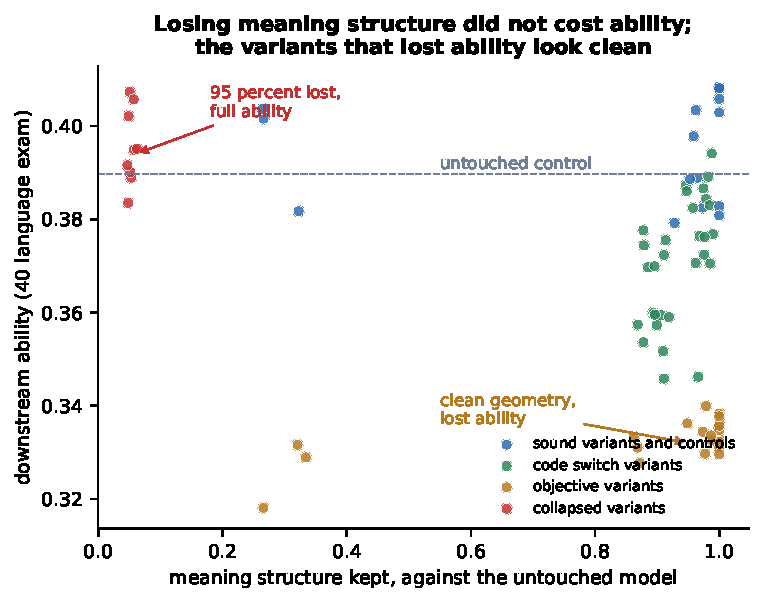
\includegraphics[width=\linewidth]{fig2_collapse_benign.pdf}
\end{column}
\end{columns}
\vspace{4pt}
{\color{mut}Representational damage and capability damage are
separable. That was not the working assumption.}
\end{frame}

% ---------------------------------------------------------------- 8
\begin{frame}{So what should a metric report?}
\large
If one number can hide a 95 percent loss, and if geometric health does
not imply capability, then no single score is safe.
\vspace{16pt}

\normalsize
\Hi{RMFS reports four readings per language, side by side.}
\vspace{8pt}
\begin{itemize}\setlength\itemsep{5pt}
\item \textbf{Meaning against language} --- LFS's original
decomposition, kept intact
\item \textbf{Sentence matching} --- can the model find a sentence's
translation among distractors
\item \textbf{Weakest aligned languages} --- behaviour in the poorest
aligned tail, where training damage appears first
\item \textbf{Collapse flag} --- meaning structure against a reference
checkpoint, for training settings
\end{itemize}
\vspace{10pt}
{\color{mut}They are kept apart because each one predicts something the
others miss. The next slide is that claim, measured.}
\end{frame}

% ---------------------------------------------------------------- 9
\begin{frame}{Each reading is worth something different}
\begin{center}
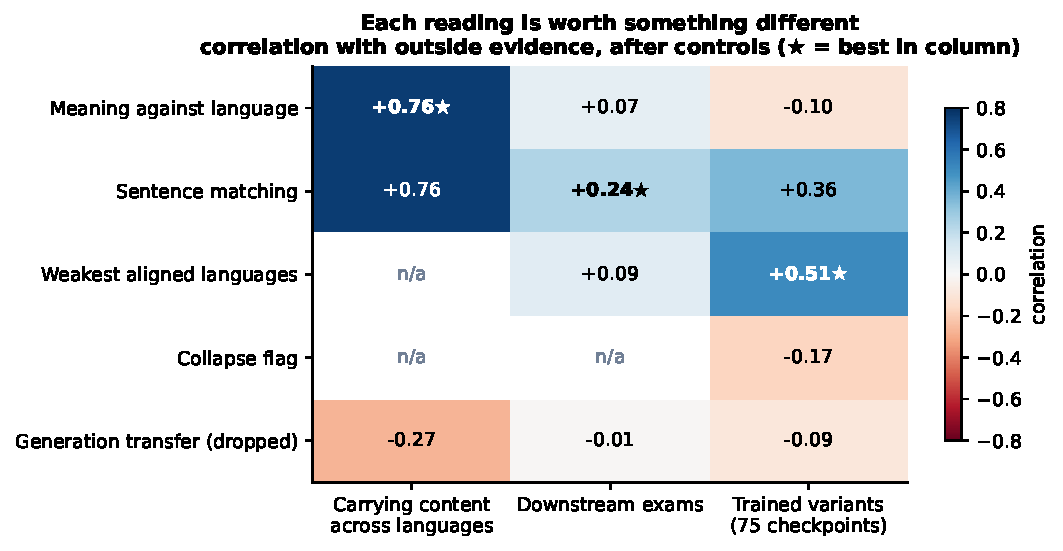
\includegraphics[width=0.82\linewidth]{fig1_validity_matrix.pdf}
\end{center}
\vspace{-6pt}
{\small Correlations after removing training data volume, language
family, script and tokenizer effects. \Hi{No reading wins twice} ---
which is the argument against averaging them into one score.}
\end{frame}

% ---------------------------------------------------------------- 10
\begin{frame}{How a score is computed}
\begin{center}
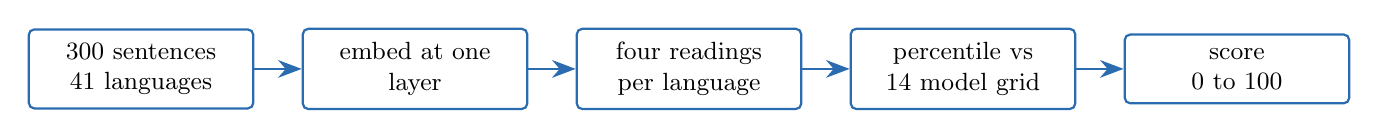
\begin{tikzpicture}[node distance=6mm,
  box/.style={draw=acc,thick,rounded corners=2pt,align=center,
              inner sep=5pt,text width=2.5cm,font=\small},
  ar/.style={-{Stealth[length=3mm]},acc,thick}]
\node[box] (a) {300 sentences\\41 languages};
\node[box,right=of a] (b) {embed at one\\layer};
\node[box,right=of b] (c) {four readings\\per language};
\node[box,right=of c] (d) {percentile vs\\14 model grid};
\node[box,right=of d] (e) {score\\0 to 100};
\draw[ar] (a)--(b); \draw[ar] (b)--(c); \draw[ar] (c)--(d);
\draw[ar] (d)--(e);
\end{tikzpicture}
\end{center}
\vspace{6pt}
\begin{itemize}\setlength\itemsep{5pt}
\item About \Hi{four GPU minutes} per model
\item Each reading is converted to its percentile against a frozen
reference grid of 14 models, then averaged
\item A score of \Hi{74} means better than 74 percent of the reference
models
\item Reported per language; the model score is the median across
languages
\end{itemize}
\vspace{6pt}
{\color{mut}Percentiles rather than raw values, because the four
readings live on different scales and averaging raw scales is what
hides damage.}
\end{frame}

% ---------------------------------------------------------------- 11
\begin{frame}{The scoreboard}
\begin{center}\large
\begin{tabular}{lc@{\hspace{2cm}}lc}
\toprule
Qwen3-8B & \Hi{90.5} & Falcon3-7B & 50.0\\
Qwen3-4B & \Hi{85.7} & OLMo-2-7B & 50.0\\
Qwen3-1.7B & 73.8 & EuroLLM-1.7B & 45.2\\
Salamandra-7B & 69.0 & bloom-1b7 & 42.9\\
bloom-7b1 & 54.8 & SmolLM2-1.7B & 35.7\\
Qwen3-0.6B & 54.8 & Mistral-7B & 33.3\\
 & & OLMo-2-1B & 28.6\\
\bottomrule
\end{tabular}
\end{center}
\vspace{10pt}
\begin{itemize}
\item Scale ordering within a family falls out with no tuning
\item Multilingual focused models sit above English centric ones of the
same size
\end{itemize}
\end{frame}

% ---------------------------------------------------------------- 12
\begin{frame}{Is the mapping between languages linear?}
Across \Hi{1{,}792} model and language pairs, fitting a ladder of maps
from simplest to most complex and selecting the simplest that is not
beaten:
\vspace{10pt}
\begin{center}\large
\begin{tabular}{lc}
\toprule
linear or simpler & \Hi{74 percent}\\
linear exactly & 60 percent\\
needs a nonlinear map & 26 percent\\
\bottomrule
\end{tabular}
\end{center}
\vspace{12pt}
\begin{itemize}\setlength\itemsep{5pt}
\item The nonlinear cases are \Hi{concentrated, not spread}: three
models (Falcon3-7B, OLMo-2-1B, OLMo-2-7B) carry 80 percent of them
\item Across the other eleven models, only \Hi{6.5 percent} of
languages need a nonlinear map
\end{itemize}
\vspace{6pt}
{\color{mut}An answer to 3.1.1 as a distribution rather than a single
case.}
\end{frame}

% ---------------------------------------------------------------- 13
\begin{frame}{A measure built on generation can run backwards}
\begin{columns}[T]
\begin{column}{0.52\textwidth}
\vspace{4pt}
A transfer measure taken from the generation harness \emph{rises} under
mild damage, and falls only when the correspondence between languages
is destroyed outright.
\vspace{10pt}
\begin{itemize}\setlength\itemsep{4pt}
\item Seen in trained variants
\item Reproduced in dose controlled distortions
\item Confirmed across models
\end{itemize}
\vspace{10pt}
{\color{mut}Impoverished representations lean harder on whatever
context they are given, so a measure that injects context rewards the
damage it should detect. This reading was dropped from the score.}
\end{column}
\begin{column}{0.48\textwidth}
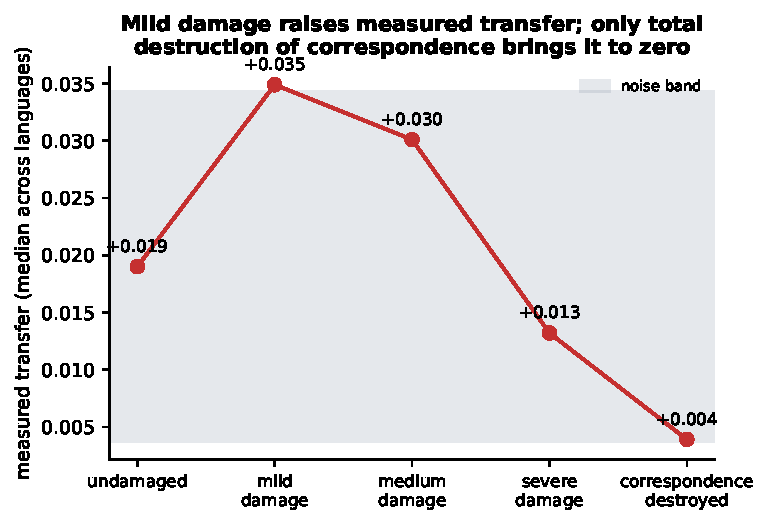
\includegraphics[width=\linewidth]{fig3_T_inversion.pdf}
\end{column}
\end{columns}
\end{frame}

% ---------------------------------------------------------------- 14
\begin{frame}{What the numbers rest on}
\begin{itemize}\setlength\itemsep{9pt}
\item \Hi{Downstream prediction sits near 0.3 after controls} --- for
every measure in this area, ours included. Raw correlations are much
higher, and are mostly training data volume.
\item \Hi{The 0.76 holds under language family resampling}
(0.60 to 0.89) but rests on four models in that comparison: treating
models as the unit gives 0.12 to 0.84.
\item \Hi{A panel of 69 languages carries the independent evidence of
roughly two.} Languages are so mutually correlated that nominal sample
size overstates the evidence by an order of magnitude.
\end{itemize}
\vspace{10pt}
{\color{mut}The third point bounds what any measure in this area can
claim from per language correlations, including this one.}
\end{frame}

% ---------------------------------------------------------------- 15
\begin{frame}{How the work was checked}
\begin{columns}[T]
\begin{column}{0.55\textwidth}
\vspace{2pt}
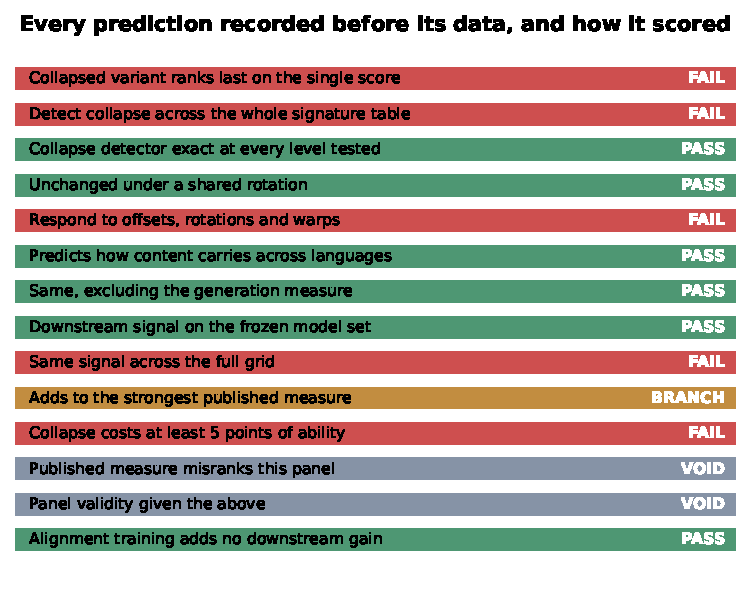
\includegraphics[width=\linewidth]{fig4_prediction_ledger.pdf}
\end{column}
\begin{column}{0.45\textwidth}
\vspace{10pt}
\begin{itemize}\setlength\itemsep{7pt}
\item Every prediction was recorded and frozen \Hi{before} the data it
referred to existed
\item Distortions with closed form answers set the tolerances
\item Correlations are confound controlled, with intervals from
resampling whole languages
\item Validity was also measured on a panel that \Hi{contains} the
damaged models
\end{itemize}
\vspace{8pt}
{\color{mut}The failures are on the slide with the passes.}
\end{column}
\end{columns}
\end{frame}

% ---------------------------------------------------------------- 16
\begin{frame}{Against Aim 1's questions}
\small
\begin{tabular}{p{0.27\textwidth}p{0.66\textwidth}}
\toprule
\textbf{3.1.1} strength of the language component; linear or more
complex &
Quantified across 14 models. Linear or simpler in 74 percent of model
and language pairs, with nonlinear cases concentrated in three models.\\
\addlinespace
\textbf{3.1.2} logit lens &
Covered in the earlier phase; carried as context.\\
\addlinespace
\textbf{3.1.3} transfer in generation &
Harness built and validated; control patches reproduce the reference
exactly. Supplies one of the three kinds of outside evidence, and
produced the inversion result.\\
\addlinespace
\textbf{3.1.4} intrinsic measures that correlate with extrinsic ones &
Measured against three kinds of outside evidence with confound
controls, and the same analysis bounds how much independent evidence a
language panel carries.\\
\bottomrule
\end{tabular}
\end{frame}

% ---------------------------------------------------------------- 17
{\setbeamercolor{background canvas}{bg=ink}
\begin{frame}
\vspace{20pt}
\color{white}\Large
\begin{itemize}\setlength\itemsep{14pt}
\item A model lost 95 percent of its meaning structure, scored best on
the metric meant to catch it, and lost no ability.
\item The measures that see representational damage and the measures
that see capability damage are \emph{not the same measures}.
\item RMFS reports four readings, each validated against different
outside evidence, scored 0 to 100 against a reference grid.
\end{itemize}
\end{frame}}

\end{document}
